\documentclass{elsarticle}
\usepackage{graphicx}
%\usepackage{multicol}
%\usepackage{footmisc}
\usepackage{amstext}
\usepackage{amsmath}
\usepackage{amssymb}
\usepackage{amsthm}
\usepackage[english]{babel}
%\usepackage[official,right]{eurosym}
\selectlanguage{english}
% Ampersand -----------------------------------------------------------

\def\id#1{\text{\em #1\/}}
\newcommand{\code}[1]{\text{\tt\small #1}}
\newcommand{\stmtText}[1]{``{\small\tt #1}''}
\newcommand{\dom}[1]{\id{dom}(#1)}
\newcommand{\cod}[1]{\id{cod}(#1)}
\renewcommand{\int}[2]{\id{inter}(#1,#2)}
\newcommand{\pop}[1]{\id{pop}(#1)}
\newcommand{\src}[1]{\id{src}(#1)}
\newcommand{\trg}[1]{\id{trg}(#1)}
\newcommand{\powerset}[1]{\cal{P}\{#1\}}
\newcommand{\theCode}{\url{http://cs.ru.nl/~B.Joosten/ampTypes/}}
\newcommand{\la}{\langle}
\newcommand{\ra}{\rangle}
\newcommand{\full}{V}
\newcommand{\declare}[3]{\id{#1}_{\pair{\id{\small #2}}{\id{\small #3}}}}
\newcommand{\fullt}[2]{V_{\pair{#1}{#2}}}
\newcommand{\iden}[1]{I}
\newcommand{\ident}[1]{I_{\id{\small #1}}}
\newcommand{\expr}[3]{(#1)_{#2\times #3}}
\newcommand{\pair}[2]{\la{#1},{#2}\ra}
\newcommand{\atom}[1]{{\tt\small #1}}
\newcommand{\atoms}{\mathcal{A}}
\newcommand{\concepts}{\mathcal{C}}
\newcommand{\decls}{\mathcal{D}}  %% names of relations
\newcommand{\rels}{\mathcal{R}}   %% all relations
\newcommand{\relations}{\mathcal{M}} % representing terms. M is a subset of R.
\newcommand{\terms}{\mathcal{T}}
\newcommand{\vertices}{N}
\newcommand{\rules}{\mathcal{H}}
\newcommand{\tf}[1]{\mathfrak{T}(#1)}
\newcommand{\ptf}[1]{\mathfrak{T}'(#1)}
\newcommand{\ti}[1]{\mathfrak{I}(#1)}
\newcommand{\tic}[1]{I_{\cal C}(#1)}
\newcommand{\relAdd}{\dagger}
\newcommand{\flip}[1]{{#1}^\smallsmile} %formerly:  {#1}^\backsim
\newcommand{\kleeneplus}[1]{{#1}^+}
\newcommand{\kleenestar}[1]{{#1}^*}
\newcommand{\cmpl}[1]{\overline{#1}}
\newcommand{\rel}{\times}
\newcommand{\compose}{;}
\newcommand{\subs}{\subseteq}%{\models}
\newcommand{\fun}{\rightarrow}
\newcommand{\isa}{\preceq}
%\newcommand{\isaClos}{\sqsubseteq}
\newcommand{\typetest}{?}
\newcommand{\meet}{\sqcap}
\newcommand{\join}{\sqcup}
\newcommand{\Meet}{\bigsqcap}
\newcommand{\Moin}{\bigsqcup} % because LaTeX has already defined command \Join.
\newcommand{\order}{\ominus}
\newcommand{\anything}{\top}
\newcommand{\nothing}{\bot}
\newcommand{\rewriteto}{\rightarrow}
\newcommand{\calc}{\implies}
\newcommand{\alland}{\bigwedge}
\newcommand{\mph}[3]{#1_{#2\times #3}}
\newcommand{\mphu}[1]{#1_{\univ\times\univ}}

%-----------------------------------------
\newcommand{\kse}{\hspace*{1.7em}}
\newcommand{\ksf}{\hspace*{1em}}
\newcommand{\ksg}{\hspace*{1em}}
\newenvironment{derivation}{\begin{tabbing}\kse \= \ksf \= \ksg \= \kill}{\end{tabbing}}
\newtheorem{definition}{Definition}
\newcommand{\term}[1]{\>\>\(#1\)\\[1ex]}
\newcommand{\rela}[2]{\>\(#1\)\>\>\{ \ #2 \ \}\\[1ex]}
\newcommand{\weg}[1]{}

\def\define#1{\label{dfn:#1}{\em #1}\index{#1}}
\def\definem#1{\label{dfn:#1}{\em #1}\index{#1}\marge{#1}}
\newcommand{\marg}[1]{\index{#1}\marge{#1}}

\hyphenation{ExecEngine}
\newtheorem{lemma}{Lemma}
\def\id#1{\text{\em #1\/}}
\def\Events{{\mathit E}}
\begin{document}

\title{A Theory for Database Transactions with no Database}
\author[ou,ordina]{Stef Joosten\fnref{fn1}}
\ead{stef.joosten@ou.nl}
\author[utwente]{Sebastiaan Joosten\fnref{fn2}}
\address[ou]{Open Universiteit Nederland, Postbus 2960, 6401 DL Heerlen, the Netherlands}
\address[ordina]{Ordina NV, Nieuwegein, the Netherlands}
\address[utwente]{University of Twente, Enschede, the Netherlands}
\fntext[fn1]{ORCID 0000-0001-8308-0189}
\fntext[fn2]{ORCID 0000-0002-6590-6220}

\begin{abstract}
	How can we make transactions work in distributed information systems without a shared database?
	Transaction theory as we know it assumes a shared data space.
	Multiple processes are acting simultaneously, each making changes to that shared data space.
	The observation that transaction mechanisms in NoSQL databases are not common
	makes us feel that a solution to this problem is not so obvious.

	This contribution proposes a theory of database transactions without a shared data space.
	This makes transactions suitable for more databases than just relational ones.
	The soundness of the theory has been established by means of formal proof.
	To show that the theory works, the theory is demonstrated by a prototype developed in Ampersand\footnote{\tt https://github.com/AmpersandTarski/Ampersand}.
	To demonstrate that the theory is about real transactions, this contribution defines semantics of conventional database transactions.
	To fulfill our promise, we also gives semantics of transactions on the semantic web.
\end{abstract}

\begin{keyword}
relation algebra\sep software development\sep legal reasoning\sep information systems design\sep Ampersand\sep MirrorMe\sep reactive programming
\end{keyword}
\maketitle

\section{Introduction}
\label{sct:Introduction}
	A distributed information system (DIS) serves its users by registering data, guarding the consistency, protecting the data,
	and providing that data accurately and meaningfully for its intended purpose.
	Users want predictable behaviour when they are simultaneously changing a shared state (e.g.\ flight reservation).
	For that purpose a transaction mechanism preserves system-wide invariants.
	Many transaction mechanisms are known that presume a shared database [refs].
	However, shared databases are not always an option in distributed cloud architectures.
	Globally distributed applications such as Netflix and LinkedIn cannot afford to rely on a shared database for obvious reasons of performance and reliability.
	Many cloud applications use distributed storage models instead.
	Examples are event stores (e.g.\ Kafka), triple stores (e.g.\ semantic web), graph databases (e.g. Neo4J) and others.
	These so-called NoSQL databases often lack functionality for transactions.
	For the purpose of doing transactions in a non-transactional situation, several architectural patterns exist.
	Some of these patterns simply circumvent the problem.
	Others will isolate transactionality into a smaller sub-problem.
	Still others introduce locking mechanisms to do the job.
	Yet, in the world of event-driven distributed systems, a dire need is felt for a theory that brings what transactions do for shared databases.
	
	This paper presents such a theory.
	It describes transactions without the assumption of a shared database.
	In this theory we express the characteristic properties of transactions: Atomicity, Consistency, Isolation, and Durability.
	{\em Atomicity} means that a sequence of primitive actions can be executed as though it were a single action.
	{\em Consistency} means that integrity rules are warranted by the database management system.
	{\em Isolation} means that actions can be done without any knowledge of what other users are doing simultaneously.
	{\em Durability} means that the contents of a database cannot change unintendedly.
	To motivate this theory, let us formulate requirements to characterize a DIS:

\section{Related work}
\label{sct:Related work}
\cite{Foster17c}

\section{Events}
\label{sct:Events}
	We need the notion of {\em event}\footnote{Cambridge Dictionary defines ``event'' as: anything that happens} to describe things that happen in a DIS.
	Let us study the requirements for events in formal terms.
	In this work we use variables $e$, $e_1$, and $e_2$ to represent events.
	Let $\mathbb E$ represent the set of all conceivable events.

	For the purpose of discussing history, we introduce a structure that represents a history at one moment in time.
	A {\em historic structure} is a tuple $\la \Events, \id{prec}\ra$ in which
\begin{eqnarray}
	&&\id{prec}\ \subseteq\ \Events\times\Events\label{req:precInE}\\
	&&(e,e)\notin\id{prec}\label{req:prec irreflexive}\\
	&&(e_1,e_2)\in\id{prec}^+\ \wedge\ (e_2,e_1)\in\id{prec}^+\ \Rightarrow\ e_1=e_2\label{req:precPlus asy}
\end{eqnarray}
	Let set $\Events$ represent all events that the DIS has registered up to some point in time.
	So for every event $e\in\Events$ we can say that it has happened (at some time in the past).
	Let $e_1\ \id{prec}\ e_2$ represent the fact that event $e_1$ has happened before event $e_2$,
	making $\id{prec}$ a relation on events in $\Events$.
	For this reason, requirement~\ref{req:prec irreflexive} excludes the situation that $e$ has happened before itself.
	To represent time faithfully, we require that $\la\Events,\id{prec}^*\ra$ is a partially ordered set,
	meaning that $\id{prec}^*$ is reflexive, transitive, and antisymmetric.
	For this reason equation~\ref{req:precPlus asy} requires the transitive closure $\id{prec}^+$ to be antisymmetric.
	In the sequel, we will use predicate $\id{HS}\la \Events, \id{prec}\ra$
	to denote that $\la \Events, \id{prec}\ra$ is a historic structure
	and we will use variables $h$ and $h'$ to denote historic structures.

	In a historic structure $\la \Events, \id{prec}\ra$, an event $e$ that precedes another event is called a {\em past} event,
	which we define as \ $\exists e_1\in\Events: e\ \id{prec}\ e_1$.
	All other events are called {\em current} events in that historic structure.

	The special case in which $\id{prec}^*$ is a total order is called a {\em linear historic structure}.
	Note that any nonempty linear historic structure has one current event.
	Other historic structures may have more.
	In a linear historic structure, every event except the first one has precisely one preceding event.
	In general, however, events may have multiple preceding events and multiple succeeding events.

	We describe each time an event $e$ happens as a mapping, $\id{happens}_{P,e}$, from one historic structure to another:
\begin{equation}
	\id{happens}_{P,e}(\la \Events, \id{prec}\ra)\ =\ \la \Events\cup\{e\}, \id{prec}\cup\{(e_1,e) | e_1\in P\}\ra
\label{req:def happens}
\end{equation}
	This happening adds one event to $\Events$ and enlarges relation $\id{prec}$ with one pair for every immediate predecessor of $e$.
	The immediate predecessors of $e$ are specified in set $P$, which we call the predecessor set.
	We need the predecessor set to cater for the distributed nature of a DIS.

\begin{lemma}
\label{lemma:happens preserves historic structure}
	If $h=\la \Events, \id{prec}\ra$ is a historic structure and $P\subseteq\Events$ and $e\notin\Events$
	then $\id{happens}_{P,e}(h)$ is a historic structure.
\end{lemma}
	Lemma~\ref{lemma:happens preserves historic structure} says that $\id{happens}_{P,e}$ preserves the historic structure.
	This lemma has been proven in proof assistant Isabelle/HOL.
	To understand why $P\subseteq\Events$ is necessary,
	let $\la \Events', \id{prec}'\ra=\id{happens}_{P,e}(h)$.
	Now suppose event $e_1\in P$ but $e_1\notin\Events$.
	Equation~\ref{req:def happens} tells us that $(e_1,e)\in\id{prec}'$.
	However, this violates requirement~\ref{req:precInE}.
	So it is necessary that every $e_1\in P$ is an element of $\Events$.
	Similarly, $e\notin\Events$ is a necessary condition,
	because any $e\in\Events$ violates the antisymmetry of $\id{prec}^+$ (requirement~\ref{req:precPlus asy}).

	Together with an empty historic structure, $\la \emptyset, \emptyset\ra$,
	we can define a historic structure recursively by means of $\id{happens}$:
\begin{eqnarray}
	&&\id{HS}\la \emptyset, \emptyset\ra\label{def:zeroHS}\\
&&\begin{array}{@{}l}
	P\subseteq\Events\ \wedge\ e\notin E\ \wedge\ \id{HS}\la \Events, \id{prec}\ra\ \Rightarrow\ \id{HS}(\id{happens}_{P,e}\la \Events, \id{prec}\ra)
\end{array}
\label{req:recursive def happens}
\end{eqnarray}
	Equation~\ref{def:zeroHS} says that $\la \emptyset, \emptyset\ra$ is a historic structure.
	Equation~\ref{req:recursive def happens} specifies recursively that $\id{happens}_{P,e}(h)$ is a historic structure iff
	$h$ is a historic structure and if $P$ and $e$ satisfy the specified conditions.
	This definition allows us to prove properties of finite historic structures by induction.
	In practical situations, every historic structure is finite.

	Note that $\id{happens}_{P,e}$ can make current events become past events.
	If $h'=\id{happens}_{P,e}(h)$, every event in $P$ becomes a past event in $h'$ and event $e$ becomes current in $h'$.

	Let $h$ and $h'$ be historic structures.
	We use the subset symbol $\subseteq$ to represent the fact that $h$ is a {\em historic substructure} of $h'$.
	This is defined as:
\begin{equation}
\label{def:historic substructure}
	\la \Events, \id{prec}\ra\ \subseteq\ \la \Events', \id{prec}'\ra\ \Leftrightarrow\ \Events\subseteq\Events'\ \wedge\ \id{prec}\subseteq\id{prec}'
\end{equation}
	Note that $\id{happens}_{P,e}(h)=h'$ implies that $h\subseteq h'$.

	Having defined historic structures and the way they grow, let us proceed to determine requirements for states.

\section{States}
	This section defines the requirements for predictable behavior of a distributed information system (DIS).
	We consider behavior to be predictable if every state can be computed unambiguously from its history.
	So let us introduce the notion of state.

	Let $\mathbb S$ represent the set of all conceivable states.
	A {\em stateful historic structure} is a triple $\la\Events, \id{prec}, \id{state}\ra$ in which
	$\la \Events, \id{prec}\ra$ is a historic structure and $\id{state}:\Events\rightarrow{\mathbb S}$ is a function
	that maps every event in $\Events$ to a state.
	We will use predicate $\id{SHS}\la \Events, \id{prec}, \id{state}\ra$
	to express that $\la \Events, \id{prec}, \id{state}\ra$ is a stateful historic structure.
	Let $s=\id{state}(e)$ represent the fact that $s$ is the state immediately after event $e$ has happened.
	Or shorter: $s$ is the state after event $e$.
	Instead of $s=\id{state}(e)$, we may also write $(s,e)\in\id{state}$ because a function is a univalent and total relation
	(and therefore a set of pairs).
	A {\em current state} is the state after a current event
	and a {\em past state} is the state after a past event.

	In a stateful historic structure, the occurrence of an event $e$ defines a new historic structure.
	This is the way systems evolve over time.
	So we define the occurrence of an event as a mapping, $\id{occurs}_{P,e,s}$, from one SHS to another SHS:
\begin{equation}
\begin{array}{l}
	\id{occurs}_{P,e,s}(\la \Events, \id{prec}, \id{state}\ra)\\
	\ =\ \la \Events\cup\{e\},\ \id{prec}\cup\{(e_1,e) | e_1\in P\},\ \id{state}\cup\{(e,s)\}\ra
\end{array}	
\label{eqn:def occurs}
\end{equation}
	In fact, this definition expands the definition of historic structures (eqn.~\ref{req:def happens}).
	By using lemma~\ref{lemma:happens preserves historic structure} we can prove that $\id{occurs}_{P,e,s}$ preserves
	the stateful historic structure.
	Also, we will use the subset symbol $\subseteq$ to represent the fact that $h$ is a {\em stateful historic substructure} of $h'$.
	And it will come as no surprise that $\id{occurs}_{P,e,s}(h)=h'$ implies that $h\subseteq h'$.
	To describe the growth of a stateful historic structure we can define stateful historic structures recursively:
\begin{eqnarray}
	&&\id{SHS}\la \emptyset, \emptyset, \emptyset\ra\\
&&\begin{array}{@{}l}
	P\subseteq\Events\ \wedge\ e\notin E\ \wedge\ \id{SHS}\la \Events, \id{prec}, \id{state}\ra\\
	\ \ \Rightarrow\ \id{SHS}(\id{occurs}_{P,e,s}\la \Events, \id{prec}, \id{state}\ra)
\end{array}
\label{req:recursive def occurs}
\end{eqnarray}

\section{Transactions}
\label{sct:Transactions}
	Information systems can register changes (as opposed to states) to avoid duplicating most of a previous state into a new state.
	Such changes are called {\em transactions}.
	For the purpose of computing a new state ($s_2$) from a given state ($s_1$),
	we need two operators, $\oplus$ and $\ominus$, such that
\begin{equation}
	s_2\ =\ s_1\oplus(s_2\ominus s_1)
\label{req:oplus and ominus}
\end{equation}
	Let us call $s_2\ominus s_1$ the difference between states $s_2$ and $s_1$.
	In a stateful historic structure we can represent transactions by means of a function $\delta$,
	where $\delta(e_1,e_2)$ represents the change of state from event $e_1$ to $e_2$.
\begin{equation}
	\delta(e_1,e_2)\ =\ \id{state}(e_2)\ominus\id{state}(e_1)
\label{def:delta}
\end{equation}
	The transaction caused by event $e$ can be described by:
\begin{equation}
	h'=\id{occurs}_{P,e,s}(h)\ \Rightarrow\ \begin{array}[t]{@{}ll}
		\id{state}(e)\ =\ s&\wedge\\
		\forall e_1\in P: s\ =\ \id{state}(e_1)\oplus\delta(e_1,e)
	\end{array}
\label{req:transaction}
\end{equation}
	We can define transactions recursively, in which we designate one specific state,
	$\mathcal I\in\mathbb S$,
	as initial state.
\begin{equation}
\begin{array}{l}
	e\notin\Events\ \wedge\ P\subseteq\Events\ \Rightarrow\\
	\id{trans}_{P,e_1,e,\Delta}(\la\Events, \id{prec}, \id{state}\ra)\\
	\ \ =\ \begin{array}[t]{@{}l@{}c@{}ll}
		\text{Let }s_1&=&\id{state}(e_1)\text{,}&\text{if }e_1\in P\\
				&=&\mathcal I\text{,}&\text{otherwise}\\
		\multicolumn{4}{@{}l}{\text{in }\la\Events\cup\{e\}, \id{prec}\cup\{(e_2,e)|e_2\in P\}, \id{state}\cup\{(e,s_1\oplus\Delta)\}\ra}
		\end{array}
\end{array}
\label{req:recursive transaction}
\end{equation}
		

\section{Atomicity}
\label{sct:Atomicity}
	{\em Atomicity} means that a state change caused by a sequence of events can be reproduced as a single event.

	So let us first discuss event sequences.
	Let us define an event sequence as a totally ordered historic structure.
	Note that a historic structure that is not totally ordered may contain multiple historic substructures
	that are totally ordered.
	Typically, event sequences occur multiply in a historic structure.


\section{Bibliography}
\bibliographystyle{elsarticle-harv}
\bibliography{doc}


\end{document}

	\section{Threads}
	So how does a stateful historic structure represent a distributed information system?
\marginpar{claim}
	Part of the answer is that a substructure of a stateful historic structure is a stateful historic structure by itself.

	The answer is that we have made no assumptions about location,
	like for instance that there is a shared memory.
	Even if we assume that each state exists in one location,
	a stateful historic structure can still have multiple current states.
	Each of these states can exist in a separate location.

	The purpose of threads is to support deterministic computations.
	We consider any nonempty historic structure that is totally ordered to be a thread.
	A {\em thread} is a historic structure $\la \Events, \id{prec}\ra$ that satisfies
\begin{eqnarray}
	\forall e_1,e_2&:&e_1\in\Events\ \wedge\ e_2\in\Events\ \Rightarrow\ e_1\ \id{prec}+\ e_2\vee e_2\ \id{prec}^+\ e_1\label{eqn:order is total}\\
	\exists e&:&e\in\Events\label{eqn:nonempty thread}
\end{eqnarray}
	The total order (\ref{eqn:order is total}) is required to get deterministic results from a computation in a thread.
	In order to talk about the first and the last event in a thread, we require at least one event (\ref{eqn:nonempty thread}) in a thread.
	We shall use variable $t$ to represent threads.
	The first event in a thread $t$ is the infimum of the events in $t$;
	the last event is the supremum.

	We need the notion of state%
	\footnote{Cambridge Dictionary meaning of ``state'':
	a condition or way of being that exists at a particular time}
	to describe things that change over time.
	We shall use variables $s$, $s_1$, and $s_2$ to denote states.
	Let $\id{state}(e)$ represent the state after event $e$ has happened.

\section{Distributed Information System}
	
	Now equation~\ref{eqn:eval step} is the recursion step and the initial state is
	the starting point of the recursive computation of the final state of $t$.
	We consider a distributed information system as a set of processes that share a history.
	The system is distributed because processes need not share all histories.
	We need the notion of process%
	\footnote{Cambridge Dictionary meaning of ``process'':
		a series of actions that you take in order to achieve a result}
	to describe how components of a DIS interact.
	Let $\mathbb P$ be the set of all processes.
	We have formulated the following requirements:
	\begin{itemize}
	\item Belong/Contain\\
		To represent the fact that an event {\em belongs to} a process or
		(equivalently) that a process {\em contains} certain events,
		let $e\in p$ represent the statement that event $e$ belongs to process $p$.
	\item Shared history\\
		To abstract away from location, we make no assumptions with respect to the place where a process lives.
		However, to partake in a distributed system, processes must be able to share history.
		For that purpose we define what it means to be part of a history:
		\begin{equation}
			p\ \id{partof}\ h\ \Leftrightarrow\ (\forall e: e\in p\Rightarrow e\in h)
		\end{equation}
		We define an order between processes that share a history.
		\begin{equation}
			p_1\ \preceq\ p_2\ \Leftrightarrow(\forall e: e\in p_1\Rightarrow e\in p_2)
		\end{equation}
		We can prove that
		\begin{equation}
			p_1\ \preceq\ p_2\ \Rightarrow\ (\exists h:p_1\ \id{partof}\ h\wedge p_2\ \id{partof}\ h)
		\end{equation}
	\item Total order\\
		We require a process to have predictable behaviour, for which we need the process to contain a series (sequence) of events.
		So we require that $(\{e|e\in p\}, \preceq)$ is a total order.
		Apart from being a partial order, $\preceq$ must satisfy (for every $e_1$, $e_2$, and $p$):
		\begin{equation}
			e_1\in p\ \wedge\ e_2\in p\ \Rightarrow\ e_1\preceq e_2\vee e_2\preceq e_1
		\end{equation}
	\end{itemize}
	
\section{States}
	\begin{itemize}
	\item Revert\\
		A change can be used to compute a previous state.
		For this purpose we require an operator $\ominus$ such that
	\begin{equation}
		s_1\oplus\Delta=s_2\ \Leftrightarrow\ s_1=s_2\ominus\Delta
	\end{equation}
		As a consequence, we have for every event $e$:
	\begin{equation}
		\id{state}(\id{past}(e))=\id{state}(\id{pres}(e))\ominus\id{delta}(e)
	\end{equation}
		With $\preceq$ being reflexive, antisymmetric, and transitive,
		it follows immediately that $\oplus$ is idempotent, commutative, and associative.
	\end{itemize}

\section{Consistency}
\label{sct:Consistency}
	{\em Consistency} means that integrity rules are warranted by the database management system.

	If $s$ is a state and $r$ is an integrity rule, then $s\ \id{sat}\ r$ means that $s$ satisfies rule $r$
	and $s\ \overline{\id{sat}}\ r$ means that $s$ does not satisfy rule $r$.

	Let us call the set of integrity rules $\mathcal R$.
	A state $s$ is called consistent if it satisfies every integrity rule $r\in\mathcal R$
\begin{equation}
	\id{consistent}(s)\ =\ \forall r\in\mathcal R: s\ \id{sat}\ r
\end{equation}
	The system is consistent if the initial state is consistent and it can only reach consistent states by means of atomic actions.
	So all states in the history graph are consistent with $\mathcal R$.


\section{Isolation}
\label{sct:Isolation}
{\em Isolation} means that actions can be done without any knowledge of what other users are doing simultaneously.

\section{Durability}
\label{sct:Durability}
{\em Durability} means that the contents of a database cannot change unintendedly.

\section{Bibliography}
\bibliographystyle{elsarticle-harv}
\bibliography{doc}


\end{document}

%% Obsolete

\section{Consistency}
\label{sct:Consistency}
Each user of a database issues a stream of events.
	The order (in time) of events is given by a relation\footnote{%
A relation $\declare{r}{A}{B}$ is a set of tuples. Each tuple $\pair{a}{b}$ in that set satisfies $a\in A$ and $b\in B$}
	$\declare{pred}{Event}{Event}$,
	where $\pair{e1}{e2}\in\id{pred}$ means that event $e1$ precedes event $e2$.
	From a user perspective this stream is a sequence, so every event except the first has exactly one predecessor.
	
	For simplicity's sake, we assume the user sees a finite set of items at any given moment.
	The items seen by the user at any moment are given by a relation $\declare{state}{Event}{Item}$,
	where $\pair{e}{i}\in\id{state}$ means that item $i$ exists immediately after $e$ has happened.
	So the set of items visible to the user immediately after $e$ has happened can be computed by $\{ i | \pair{e}{i}\in\id{state} \}$.
	Note that the relation $\id{state}$ is interpreted in an open world.
	If $\pair{e}{i}\not\in\id{state}$ this does not mean $i$ does not exist.
	It just means that the pair $\pair{e}{i}$ is not in $\id{state}$, so the user will not see it.

	To cope with change, a user may insert and/or delete items at will.
	Let us specify these deletions and insertions by two relations, $\declare{ins}{Event}{Item}$ and $\declare{del}{Event}{Item}$,
	where $\pair{e}{i}\in\id{ins}$ means that pair $\pair{e}{i}$ is to be added to $\id{state}$,
	and $\pair{e}{i}\in\id{del}$ means that pair $\pair{e}{i}$ is to be removed from $\id{state}$.
	More precisely, let us consider an event $e$.
	The items $\{ i | \pair{e}{i}\in\id{state} \}$ are the items that exist immediately after the preceding event has happened,
	minus the items to be removed, plus the items to be inserted.
	The following equation defines this \define{behaviour}:
\begin{equation}
	\id{state}\ =\ (\id{pred};\id{state}-\id{del})\cup\id{ins}
\label{behaviour}
\end{equation}
	Equation~\ref{behaviour} says that the items visible to the user immediately after an event $e$
	are all items that are inserted together with items that were visible immediately after the preceding event, except those that were deleted.

	We define $A_{(\id{ins},\id{del})}$ as the function\footnote{The name $A$ is chosen as a reminder to the word ``action''.}
	that embodies this change:
\begin{equation}
	A_{(\id{ins},\id{del})}(x)\ =\ (x-\id{del})\cup\id{ins}
\end{equation}

	This raises the question whether we can compose two actions into a single action.
	For this, we derive:
\[\begin{array}{r@{~}l}
	&(((x-\id{del})\cup\id{ins})-\id{del}')\cup\id{ins}'\\
	=&\hspace{1in}\{x-y=x\cap\overline{y}\}\\
	&(((x\cap\overline{\id{del}})\cup\id{ins})\cap\overline{\id{del}'})\cup\id{ins}'\\
	=&\hspace{1in}\{\text{distribute $\cap$ over $\cup$}\}\\
	&(x\cap\overline{\id{del}}\cap\overline{\id{del}'})\cup(\id{ins}\cap\overline{\id{del}'})\cup\id{ins}'\\
	=&\hspace{1in}\{\text{De Morgan}\}\\
	&(x-(\id{del}\cup\id{del}'))\cup(\id{ins}-\id{del}')\cup\id{ins}'\\
	=&\hspace{1in}\{\text{Assume}\ \id{ins}\cap\id{del}=\emptyset\ \text{and}\ \id{ins}'\cap\id{del}'=\emptyset\}\\
	&(x-(\id{del}\cup\id{del}'))\cup(\id{ins}\cup\id{ins}')
\end{array}\]
	This yields composition ($;$) of $A$:
\begin{equation}
	A_{(\id{ins},\id{del})}\ ;\ A_{(\id{ins}',\id{del}')}\ =\ A_{((\id{ins}-\id{del}')\cup\id{ins}', \id{del}\cup\id{del}')}
\label{composition of A}
\end{equation}
	
	The composition operator turns out to be commutative, but under a condition.
	This will appear to be useful later on in this paper.
	Equation~\ref{composition of A} shows that we only need to investigate commutativity in the first argument of $A$: 
\[\begin{array}{r@{~}rcl}
	&A_{(\id{ins},\id{del})}\ ;\ A_{(\id{ins}',\id{del}')}&=&A_{(\id{ins}',\id{del}')}\ ;\ A_{(\id{ins},\id{del})}\\
	\Leftrightarrow\\
	&A_{((\id{ins}-\id{del}')\cup\id{ins}', \id{del}\cup\id{del}')}&=&A_{((\id{ins}'-\id{del})\cup\id{ins}, \id{del}'\cup\id{del})}\\
	\Leftrightarrow\\
	&(\id{ins}-\id{del}')\cup\id{ins}'&=&(\id{ins}'-\id{del})\cup\id{ins}\\
	\Leftrightarrow\\
	&(\id{ins}\cap\overline{\id{del}'})\cup\id{ins}'&=&(\id{ins}'\cap\overline{\id{del}})\cup\id{ins}\\
	\Leftrightarrow\\
	&(\id{ins}\cup\id{ins}')\cap(\overline{\id{del}'}\cup\id{ins}')&=&(\id{ins}\cup\id{ins}')\cap(\overline{\id{del}}\cup\id{ins})\\
	\Leftrightarrow\\
	&(\id{ins}\cup\id{ins}')-\overline{\overline{\id{del}'}\cup\id{ins}'}&=&(\id{ins}\cup\id{ins}')-\overline{\overline{\id{del}}\cup\id{ins}}\\
	\Leftrightarrow\\
	&\id{del}'\cap\overline{\id{ins}'}&=&\id{del}\cap\overline{\id{ins}}\\
	\Leftrightarrow\\
	&\id{del}'-\id{ins}'&=&\id{del}-\id{ins}
\end{array}\]
	For the purpose of making commutativity independent of its arguments,
	we must check the condition $\id{del}'-\id{ins}'=\id{del}-\id{ins}$.

\section{Isolation}
\label{sct:Isolation}
	If a user were alone,
	The moment a transaction starts, its user is isolated from other users.
	That moment is represented by a relation $\declare{beginTransaction}{Event}{Transaction}$,
	where $\pair{e}{t}\in\id{beginTransaction}$ means that event $e$ marks the start of transaction $t$.


\section{Ampersand}
\label{sct:Ampersand}
	In this section we explain the basics of Ampersand.
	The reader is expected to have sufficient background in relation algebra to understand the remainder of this paper.

	The core of an Ampersand script is a triple $\la\rules,\rels,\concepts\ra$,
	which consists of a set of rules $\rules$, relations $\rels$, and concepts $\concepts$.
	An Ampersand script is interpreted by the compiler as an information system.
	The rules constitute a theory in heterogeneous relation algebra.
	They constrain a body of data that resides in a database.

	The Ampersand compiler generates a database from relations in the script.
	A database application%
\footnote{Ampersand generates an application that consists of a relational database and interface components.
	Currently this application runs server-side on a PHP/MySQL platform and on a web-browser on the client-side.}
	assists users to keep rules satisfied throughout the lifetime of the database. It is also generated by Ampersand.

	A rule is a constraint in the form of an equality between two terms.
	Terms are built from relations.
	Ampersand interprets every relation as a finite set of pairs, which are stored in the database.
	The phase in which Ampersand takes a script and turns it into a database, is what we will refer to as \define{compile-time}.
	The phase in which a user interacts with the database, is what we will refer to as \define{run-time}.
	At run-time, Ampersand can decide which rules are satisfied by querying the database.
	The compiler generates all software needed to keep rules satisfied at run-time.
	If one of the rules is not satisfied as a result of data that has changed,
	that change is reverted (rolled back) to the original state.
	Either way, Ampersand ensures that all rules remain satisfied.
	
	Atoms are values that have no internal structure, meant to represent data elements in a database.
	From a business perspective, atoms are used to represent concrete items of the world,
	such as \atom{Peter}, \atom{1}, or \atom{the king of France}.
	By convention throughout the remainder of this paper, variables $a$, $b$, and $c$ are used to represent \emph{atoms}.
	The set of all atoms is called $\atoms$.
        Each atom is an instance of a \emph{concept}.

	Concepts (from set $\concepts$) are names we use to classify atoms in a meaningful way.
	For example, you might choose to classify \atom{Peter} as a person, and \atom{074238991} as a telephone number.
        We will use variables $A$, $B$, $C$, $D$ to represent concepts.
	The term $\ident{A}$ represents the \emph{identity relation} of concept $A$.
	The expression $a \in A$ means that atom $a$ is an \emph{instance} of concept $A$.
	The declaration of $A\isa B$ (pronounce: $A$ is a $B$)
	in an Ampersand script states that any instance of $A$ is an instance of $B$ as well.
	We call this {\em specialization}, but it is also known as {\em generalization} or {\em subtyping}.
	Specialization is needed to allow statements such as: ``An orange is a fruit that ....''.
	Specialization is not used in the remainder of this paper.

	Relations (from set $\rels$) are used in information systems to store data.
%	A \define{fact} is a statement that is true in a business context.
%	Facts are stored and kept as data in a computer.
	As data changes over time, so do the contents of these relations.
	In this paper relations are represented by variables $r$, $s$, and $d$.
	We represent the declaration of a relation $r$ by $\declare{nm}{A}{B}$,
	in which \id{nm} is a name and $A$ and $B$ are concepts.
	We call $A$ the source concept and $B$ the target concept of the relation.
	The pair $\pair{A}{B}$ is called the \emph{type} of the relation.
	The term $\fullt{A}{B}$ represents the \emph{universal relation} over concepts $A$ and $B$.

	The meaning of relations in Ampersand is defined by an interpretation function $\mathfrak{I}$.
	It maps each relation to a set of pairs.
	The type system of Ampersand guarantees that each pair in $r$ respects the type of $r$:
\begin{equation}
	\pair{a}{b}\in\ti{\declare{nm}{A}{B}} \Rightarrow\ a \in A \wedge b \in B \label{typing of relations}
\end{equation}
	The type system is strong, which means that every atom has a type.
	The type system is static, which means that type checking is entirely done at compile-time.

	Terms are used to combine relations using operators.
	The set of terms is called $\terms$.
\begin{definition}[terms]
\label{def:terms}
\item   The set of terms, $\terms$, is the smallest set that satisfies, for all $r,s \in \terms$, $d\in\rels$ and $A,B \in \concepts$: 
\begin{eqnarray}
	d&\in&\terms         \quad\quad\text{(every relation is a term)}\\
	(r \cup s)&\in&\terms\quad\quad\text{(union)}\\
	(r \cap s)&\in&\terms\quad\quad\text{(intersection)}\\
	(r-s)&\in&\terms     \quad\quad\text{(difference)}\label{def:difference}\\
	(r;s)&\in&\terms     \quad\quad\text{(composition)}\\
	(r\backslash s)&\in&\terms     \quad\quad\text{(right residual)}\\
	(r\slash s)&\in&\terms     \quad\quad\text{(left residual)}\\
	\flip r&\in&\terms   \quad\quad\text{(converse)}\\
	\cmpl{r}&\in&\terms   \quad\quad\text{(complement)}\\
%	\kleeneplus r&\in&\terms   \quad\quad\text{(Kleene closure)}\\
%	\kleenestar r&\in&\terms   \quad\quad\text{(Kleene closure)}\\
	\ident{A}&\in&\terms \quad\quad\text{(identity)}\\
	\fullt{A}{B}&\in&\terms \quad\quad\text{(full set)}
\end{eqnarray}
\end{definition}
	Throughout the remainder of this paper,	terms are represented by variables $r$, $s$, $d$, and $t$.
	The \define{type} of a term $r$ is a pair of concepts, given by $\tf{r}$.
	$\mathfrak{T}$ is a partial function that maps terms to types.
	If a term has one type, it is called \define{type correct}.
	The Ampersand compiler requires all terms to be type correct.
	If no type can be assigned, the compiler gives an error message.
	If multiple types are assignable to a term, the ambiguity is signalled by the compiler.
	In that case it will also emit an error message and prompt the programmer to disambiguate the term by adding type information.
	In practice, the derivation of types can disambiguate most terms.
	So, the programmer experiences some freedom to denote distinct relations by the same name without the obligation to specify their types at all occurrences.
	The compiler does not generate any code if there is a term that is not type correct.
	The type function and its restrictions are discussed in~\cite{Joosten2015}
	and have no consequences for the remainder of this paper.

 	The meaning of terms in Ampersand is given by an interpretation function $\mathfrak{I}$.
	Let $A$ and $B$ be finite sets of atoms, then $\mathfrak{I}$ maps each term to the set of pairs for which that term stands.
\begin{definition}[interpretation of terms]
\label{interpretation of terms}
\item   For every $A,B\in\concepts$ and $r,s\in\terms$
\begin{eqnarray}
	\ti{r}		 &=&\{\pair{a}{b}|\ a\ r\ b\}	\\
	\ti{r \cup s}	 &=&\{\pair{a}{b}|\ \pair{a}{b}\in\ti{r}\ \text{or }\ \pair{a}{b}\in\ti{s}\}	\\
	\ti{r \cap s}	 &=&\{\pair{a}{b}|\ \pair{a}{b}\in\ti{r}\ \text{and}\ \pair{a}{b}\in\ti{s}\}	\\
	\ti{r-s}	 &=&\{\pair{a}{b}|\ \pair{a}{b}\in\ti{r}\ \text{and}\ \pair{a}{b}\notin\ti{s}\}	\\
	\ti{r;s}	 &=&\{\pair{a}{c}|\ \text{for some}\ b,\ \pair{a}{b}\in\ti{r}\ \text{and}\ \pair{b}{c}\in\ti{s}\}	\\
	\ti{r\backslash s}	 &=&\{\pair{b}{c}|\ \text{for all}\ a,\ \pair{a}{b}\in\ti{r}\ \text{implies}\ \pair{a}{c}\in\ti{s}\}	\\
	\ti{r\slash s}	 &=&\{\pair{a}{b}|\ \text{for all}\ c,\ \pair{b}{c}\in\ti{s}\ \text{implies}\ \pair{a}{c}\in\ti{r}\}	\\
	\ti{\flip{r}}	 &=&\{\pair{b}{a}|\ \pair{a}{b}\in\ti{r}    \}	\\
	\ti{\cmpl{\declare{r}{A}{B}}}	 &=&\fullt{A}{B}-r	\\
%	\ti{\kleeneplus{r}}	 &=&\text{the smallest set that satisfies }\kleeneplus{r}=r\ \cup\ \kleeneplus{r};\kleeneplus{r}	\\
%	\ti{\kleenestar{\declare{r}{A}{A}}}	 &=&\ident{A}\cup\kleeneplus{r}\\
	\ti{\ident{A}} 	 &=&\{\pair{a}{a}|\ a\in A\}	\\
	\ti{\fullt{A}{B}}&=&\{\pair{a}{b}|\ a\in A, b\in B\}
\end{eqnarray}
\end{definition}
%	The Kleene closure operators (postfix $\kleeneplus{\ }$ and $\kleenestar{\ }$) have been implemented partially in the current Ampersand implementation.

	A \define{rule} is a pair of terms $r,s\in\terms$ with $\tf{r}=\tf{s}$, which is syntactically recognizable as a rule.
\[\text{RULE}\ r = s\]
	This means \(\ti{r} = \ti{s}\). In practice, many rules are written as:
\[\text{RULE}\ r\subs s\]
	This is a shorthand for 
\[\text{RULE}\ r\cap s = r\]
	We have enhanced the type function $\mathfrak{T}$ and the interpretation function $\mathfrak{I}$ to cover rules as well.
	If $\tf{r}=\tf{s}$ and $\tf{s}=\pair{A}{B}$:
\begin{eqnarray}
	\tf{\text{RULE}\ r = s}   &=&\pair{A}{B}\\
	\tf{\text{RULE}\ r\subs s}&=&\pair{A}{B}\\
 resolved this \end{eqnarray}

	We call a rule $\text{RULE}\ r = s$ \define{satisfied} when its interpretation equals $\ti{\fullt{A}{B}}$.
	As the population of relations used in $r$ changes with time, the satisfaction of the rule changes accordingly.
	A software developer, who conceives these rules, must consider how to keep each one of them satisfied.
	We call a rule \define{violated} if it is not satisfied.
	The set $\ti{(s-r)\cup(r-s)}$ is called the \emph{violation set} of \(\text{RULE}\ r = s\).
	To \define{resolve} violations means to change the contents of relations such that the rule is satisfied%
\footnote{To \define{restore invariance} is sometimes used as a synonym to resolving violations.
	To \define{preserve invariance} is sometimes used as a synonym to keeping a rule satisfied.}.
	Consequently, such a rule may also be referred to as \define{invariant}.
	Some ways of resolving violations are presented in section~\ref{sct:Code Fragments}.
	Each pair in the violation set of a rule is called a violation of that rule.

	The software developer must define how to resolve violations when they occur.
	She does so by inserting and/or deleting pairs in appropriately chosen relations.
	Whatever choice she makes, she must ensure that her code yields data that satisfies the rules.
	When we say: ``rule $r$ specifies this action'' we mean that satisfaction of rule $r$ is a postcondition of any action specified by rule $r$. 

\section{Software for Legal Reasoning}
\label{sct:Conceptual analysis}

% \begin{figure}[htb]
% \begin{center}
%   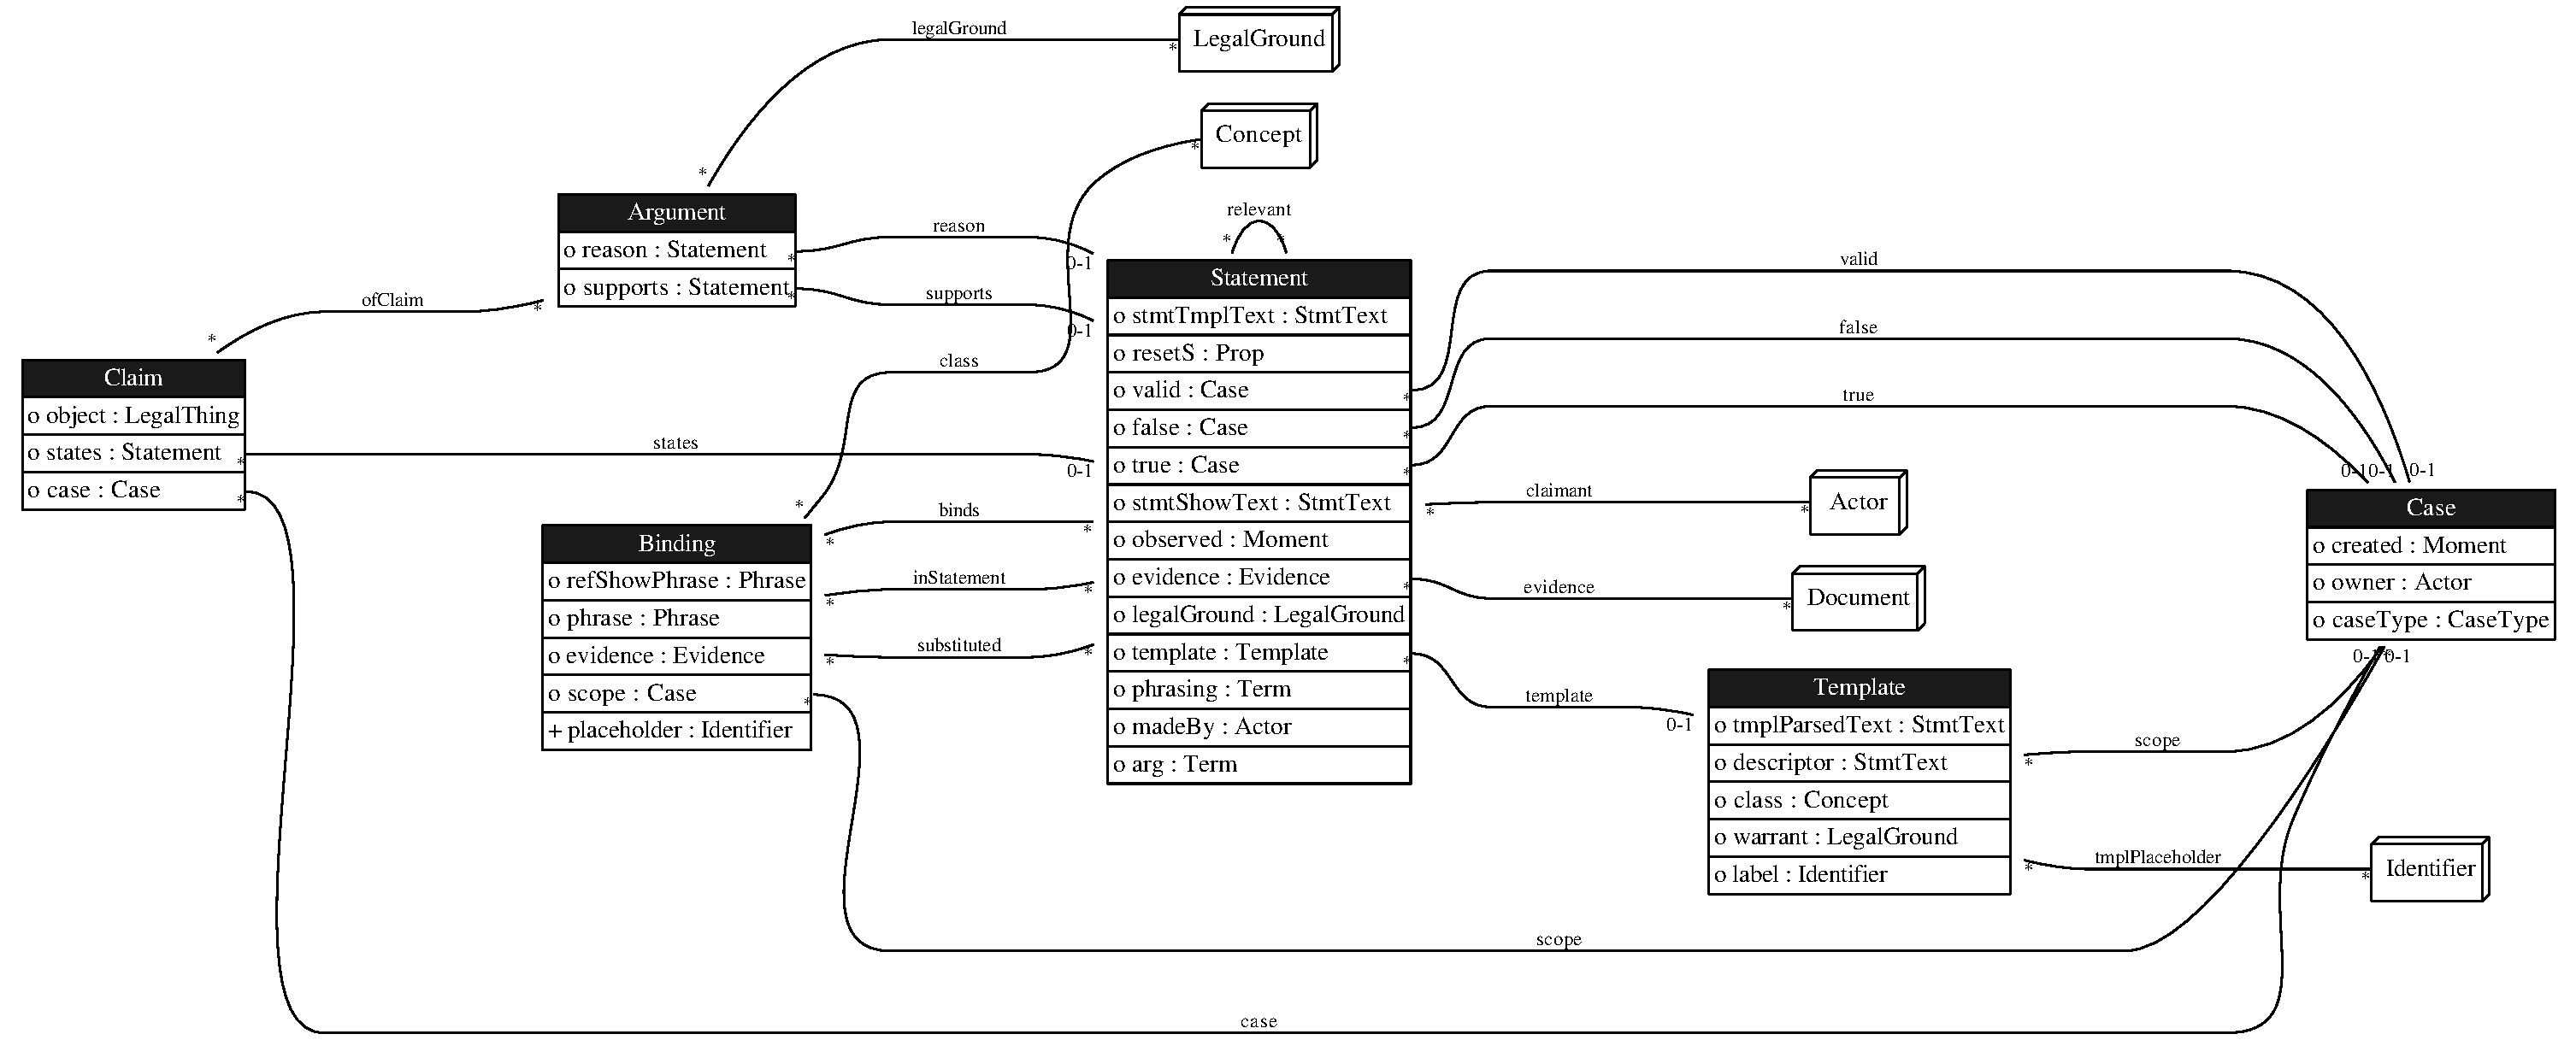
\includegraphics[angle=90,scale=.357]{LogicalDataModel.pdf}
% \end{center}
% \caption{Conceptual data model (from section~\ref{sct:Conceptual analysis})}
% \label{fig:conceptual model}
% \end{figure}

\section{Bibliography}
\bibliographystyle{elsarticle-harv}
\bibliography{doc}


\end{document}
